\documentclass{beamer}
\usepackage[utf8]{inputenc}
\usepackage[T1]{fontenc}
\usepackage[english]{babel}
\usepackage{graphicx}
\usepackage{times}

\usetheme{AGH}

\title[Technologie mobilne]{Broadcast receivers, content providers, services, async tasks}

\author[M. Nowotyński, M.Moskal, K. Osuch]{Mateusz Nowotyński \and Marcin Moskal \and Kamil Osuch}

\date[12.12.2017]{12.12.2017}

%\setbeamertemplate{itemize item}{\textbullet}

\begin{document}

{
%\usebackgroundtemplate{
\includegraphics[width=\paperwidth]{titlepage}} % wersja angielska
\usebackgroundtemplate{
\includegraphics[width=\paperwidth]{titlepagepl}} % wersja polska
 \begin{frame}
   \titlepage
 \end{frame}
}

%---------------------------------------------------------------------------


\begin{frame}{Broadcast Receivers}

\begin{block}{Do czego to służy?}
BroadcastReceiver pozwala nam na odbieranie powiadomień (Systemu bądź innej aplikacji) wewnątrz naszej aplikacji. Takim powiadomieniem może być na przykład informacja o nowej wiadomości SMS bądź rozładowanej baterii.
\end{block}
\end{frame}

\begin{frame}{Tworzenie Broadcast Receiver'a}
	Żeby zbudować nasz własny BroadcastReceiver musimy wykonać dwie czynności:
	\begin{enumerate}
		\item Stworzyć podklasę klasy BroadcastReceiver
		\item Wyspecyfikować receiver w manifeście aplikacji
	\end{enumerate}
\end{frame}

\begin{frame}{Przykład klasy Broadcast Receiver'a}
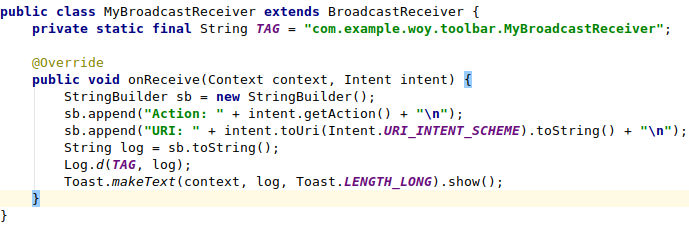
\includegraphics[width=\textwidth]{receiver}
\end{frame}

\begin{frame}{Dodanie do manifestu}
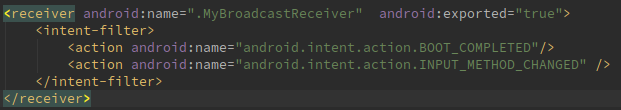
\includegraphics[width=\textwidth]{manifest}
\end{frame}

\end{document}

